\documentclass{entcs}

%% For those who don't have entcs...
%\documentclass{article}
%\newenvironment{frontmatter}{}{\maketitle}
%\newenvironment{keyword}{\begin{quote}}{\end{quote}}
%\newcommand{\thanksref}[1]{}
%\newcommand{\address}[1]{#1}
%\newtheorem{defn}{Definition}

%NOTE: oz.sty clashes with entcs.cls, so we use a hacked version of oz.sty
\usepackage{czt}
\usepackage{graphicx}
\usepackage{url}

% Extra general macros for this paper.

% Extra math-mode macros for this paper.
% Some of these may eventually go into czt.sty
\newcommand{\V}{\mathcal{V}}
\newcommand{\Zc}{Z_C}
\newcommand{\sexprUnfoldsTo}{\mathrel{=_{se}}}
\newcommand{\declListUnfoldsTo}{\mathrel{=_d}}
\newcommand{\unprefix}{\mathrel{unprefix}}
\newcommand{\schemaEquals}{\mathrel{=_S}}

\def\lastname{Utting, Malik and Toyn}

\begin{document}
\begin{frontmatter}
  \title{Transforming Z with Rules}
  \author{Mark Utting\thanksref{emailMark}}
  \address{Department of Computer Science\\
    The University of Waikato\\
    Hamilton, New Zealand} 
  \author{Petra Malik\thanksref{emailPetra}}
  \address{Department of Computer Science\\
    The University of Waikato\\
    Hamilton, New Zealand} 
  \author{Ian Toyn\thanksref{emailIan}}
  \address{Department of Computer Science\\
    The University of York\\
    Heslington, York, UK}
  \thanks[emailMark]{Email: \texttt{marku@cs.waikato.ac.nz}}
  \thanks[emailPetra]{Email: \texttt{petra@cs.waikato.ac.nz}}
  \thanks[emailIan]{Email: \texttt{ian@cs.york.ac.nz}}
\begin{abstract}
  This paper describes an extension of Z that allows transformation
  and reasoning rules to be written in a Z-like notation.  This gives
  a high-level, declarative way of specifying transformations of Z
  terms, which makes it easier to build new Z manipulation tools.  We
  describe the syntax and semantics of these rules, plus some example
  reasoning engines that use sets of rules to manipulate Z terms.  We
  demonstrate the utility of rules by discussing two sets of rules.
  One set defines unfolding of the schema expressions in Z.  The other
  set is used by the ZLive animator to preprocess Z expressions into a
  form more suitable for animation.
\end{abstract}
\begin{keyword}
  Z, CZT, ZedRules, reasoning, rewriting rules, theorem proving
\end{keyword}
\end{frontmatter}



\section{Introduction}

In many Z tools, schema unfolding and other Z transformations are performed
by large amounts of low-level code (for example, in C or Java) that
manipulate the syntax of Z schema expressions and return equivalent
unfolded terms.  This low-level approach is error-prone, and the code that
performs the transformations is time-consuming to write and difficult to
read.  The problem is that the core ideas of the abstract transformations are
hidden in the masses of low-level code needed to manipulate syntax trees.

This means that building new Z transformation tools is time-consuming,
requires programming skills, and also requires detailed knowledge of the
API for manipulating Z syntax trees.  In contrast, in an ideal world, it
should be quick and easy to define new Z transformations by writing them in
the Z notation itself, in a high-level, declarative style that is easily
understood and can perhaps even be proven correct according to some given Z
logic.  A high-level notation such as this gives better support for the
capture and reuse of the knowledge implicit in the
rules~\cite{armour:business-model00}.

This paper proposes such a declarative notation, called ZedRules.  It
allows inference rules and rewrite rules to be written in a Z-like
notation.  Within rules, the standard Z notation~\cite{ISOZ} is extended to
allow \emph{jokers} that can stand for arbitrary expressions, predicates,
declarations etc.

Section \ref{sec:relwork} discusses approaches to schema unfolding and
user-defined transformations in existing Z tools.  Section~\ref{sec:syntax}
describes the syntax and semantics of the ZedRules.
Section~\ref{sec:tools} describes three example reasoning engines provided
by CZT,\footnote{See \url{http://czt.sourceforge.net}.} which use the rules.
Section~\ref{sec:schemas} shows how the rules can be used to specify
unfolding and normalisation of schema expressions and
Section~\ref{sec:zlive} shows some of the rules that are used by the ZLive
animator to preprocess Z expressions and predicates.


\section{Related Work} \label{sec:relwork}

We briefly consider how other Z tools provide support for unfolding
schema expressions and for allowing users to define domain-specific
transformations of Z expressions.

CADiZ~\cite{cadiz:refman02} provides several builtin commands (programmed
in C) for performing local schema transformation, normalisation, and
unfolding steps.  A \emph{schema expansion} tactic is provided, which
combines these steps to give a comprehensive schema unfolding and
normalisation facility.  Expert users are able to define their own
transformations by writing tactics in a high-level, functional, tactic
language.  It is easy to write Z terms and patterns within tactics, which
makes the notation more familiar to Z users.  The tactics support pattern
matching (using jokers), while our ZedRules generalise this to allow
unification.

Z/EVES~\cite{zeves:98} provides a fixed set of transformation
commands, including an unfold command for normalising schema
expressions and a rewrite command that uses certain kinds of theorems
as rewrite rules.  Since users can specify these theorems in their Z
specifications, this gives a way of adding domain-specific rewrite
rules.  However, the expressivity of rewrite rules is quite restricted
compared to the ZedRules notation of this paper.

ProofPower\footnote{See the ProofPower web site,
\url{http://www.lemma-one.com/ProofPower/index/index.html}.} takes a
similar approach, but provides a much larger set of rewriting tactics,
with a variety of behaviour.  It is also possible to prove derived
inference rules, which can have similar expressiveness as the ZedRules
of this paper (with antecedents, jokers etc.).  However, such rules
are expressed in the proof notation of ProofPower (ML and HOL), rather
than in Z syntax.

Our ZedRules notation differs from the above approaches by allowing more
expressive rules to be written, and writing them in a declarative style in
a superset of Z.  As well as rewrite rules (for example, equalities), it is
possible to write general inference rules with side-conditions.  We shall
see that this is sufficiently expressive that we can write a set of rules
for unfolding schema expressions -- one of the more complex aspects of Z.
In contrast, the other Z tools use a mixture of builtin commands, rewrite
rules and specific tactics to implement schema expression unfolding.  Our
hope is that the additional expressivity of the ZedRules notation will make
it easier to specify many kinds of Z transformations, as well as being
useful for schema unfolding.

%This will make it easier to 
%develop new Z transformation tools such as test generators,
%domain checkers.

%There is a large and mature theory of rewriting
%systems~\cite{baader:rewriting06}.  Much of this can be applied to
%the rules that we write in the ZedRules notation.  


\section{Rule Syntax and Semantics} \label{sec:syntax}

This section describes the syntax and semantics of ZedRules.
We add three new kinds of Z paragraph to the Z standard notation,
one for rules, one for jokers, and one for oracles.

\subsection{Syntax}

Each rule has a single conclusion and zero or more antecedents, which are
typically just Z predicates, written in the standard Z notation.  The
informal semantics is that the conclusion is true if all the antecedents
are true.

For example, the \emph{Funct} rule from the $\V$
logic~\cite{brien:calculus-schemas-z00} might be written as follows:
\begin{zedrule}{Funct}
  \exists_1 x:f @ x.1 = e \\
  x \notfreein e
\derives
  y=f(e) \iff (e,y) \in f
\end{zedrule}

The \LaTeX\ input for this rule is:
\begin{verbatim}
\begin{zedrule}{Funct}
  \exists_1 x:f @ x.1 = e \\
  x \notfreein e
\derives
  y=f(e) \iff (e,y) \in f
\end{zedrule}
\end{verbatim}
while the Unicode form of the rule is similar to the typeset form.

It is also necessary to declare which names are metavariables
(jokers) and which syntactic roles they play.  For example, in
this $Funct$ rule, the $e,f$ and $y$ names stand for arbitrary
expressions (we call them \emph{expression jokers}), whereas the $x$
is a concrete bound variable name.  In the ZedRules notation, each
joker name must be declared before it is used in rules.  For example,
the following declarations declare $e,f$ and $y$ to be expression
jokers, $D1$ to be a joker that ranges over declaration lists, and
$v$ to be a name joker.

\begin{zedjoker}{Expr} e,f,y \end{zedjoker}
\begin{zedjoker}{DeclList} D1 \end{zedjoker}
\begin{zedjoker}{Name} v \end{zedjoker}

Most logics contain rules with side conditions, which check various
syntactic properties of the terms in the rule.  The most common
example is checking that a certain name $n$ is not free in a given
term $t$.  We write this as $n \notfreein t$.  To reason about Z in a
convenient way, it is also useful to be able to check properties of
signatures, distinguish between the different kinds of decorations on
names, etc.

The ZedRules notation provides oracles to support this kind of
reasoning.  An oracle is a magic thing that is able to decide that
certain predicates are true.  The sort of predicates an oracle can
decide is described by the zedoracle notation.  For example, the
\LaTeX\ input to describe an oracle that verifies that a name is not
free in a given expression is:
\begin{verbatim}
\begin{zedoracle}{NotFreeInOracle}
  v \notfreein e
\end{zedoracle}
\end{verbatim}
where $e$ is an expression joker and $v$ is a name joker.

We can group joker declarations, rules, and oracles together by
writing them within one Z section.  The Z standard \textbf{parent}
commands can then be used to inherit one set of rules and oracles into
another.  Note that, since joker declarations and rule and oracle
paragraphs start with \LaTeX\ commands that are not part of the Z
standard, they will be treated as narrative text by other Z tools, and
ignored.  This allows us to embed rules within Z specifications, but
retain backwards compatibility with Z tools that do not use the
ZedRules notation.

Currently, the scope of a joker is within all rule and oracle
paragraphs of the section in which it appears and of which it is an
ancestor.  In the future, we plan to declaring them locally to a rule
or oracle paragraph instead.  Global jokers are very concise (need to
be declared just once) but are less flexible because once a joker is
declared, it reserves the name for ever, and makes that name unusable
as an ordinary Z name.

\subsection{Semantics}

We describe the semantics of the rules independently of any operational
description of how rules can be used.  This allows rules to be used by many
different reasoning and rewrite engines.  Each engine may place different
restrictions on the rules that it allows, may apply rules using a variety
of operational semantics (apply once, apply exhaustively, apply to all
subterms bottom-up or top-down etc.), and may use a different
implementation technology (for example, an interpreter that applies the
rules or a compiler that transforms a set of rules into code).

We now define the semantics of a rule $R$ with antecedents $A_1
\ldots A_n$ and conclusion $C$ as follows.
\begin{defn} %{ValidRule}
  A rule $R$ is valid iff for every ground instantiation of
  all the jokers in the rule,
  \[
       A_1 \land \ldots \land A_n \implies C
  \]
  is a valid theorem according to the Z standard semantics.
\end{defn}

The authors of rules are responsible for ensuring that each rule they
write is valid according to this definition.  Proof tools are
responsible for ensuring that the derived rules produced by proofs
preserve this validity property.


\section{Tools for Rules} \label{sec:tools}

To use and test the rules, several tools have been implemented
in the CZT system.  These are useful for transforming Z in various
ways, but none of them are intended to be a general Z theorem prover, 
for three reasons:
\begin{enumerate}
\item There are already several other good theorem provers for Z, so
  developing another would simply fragment the existing small user-base
  further.
\item For practical theorem proving, it is necessary to develop a large set
  of rules (several for each Z construct), derived rules and tactics to
  automate the common styles of reasoning.  Experience shows that this
  requires several person years of theory development. 
\item The speed of the current CZT implementation of ZedRules is not
  sufficiently fast for practical reasoning.  The automated proof engines can
  apply a few hundred rules per second, which is adequate for simple unfolding
  tasks, but not adequate for heavy-duty reasoning with lots of rules --
  a good theorem prover needs to perform tens or hundreds of thousands of
  rules per second to be pleasant to use.
\end{enumerate}


\subsection{Oracles}

An oracle is Java code that is able to decide that a certain Z
predicate is true.  The given predicate may contain jokers, in which
case the oracle may provide instantiations under which the predicate
becomes true.  The answer of an oracle must be consistent with the Z
semantics: If an oracle declares a predicate to be true then, for
every ground instantiation of the jokers, this predicate must be a
valid theorem according to the Z standard semantics.

To ensure that proofs can be recorded and replayed, the answer of an
oracle should be monotonic with respect to the instantiations of
jokers.  For example, it is not acceptable for an oracle to return
true for predicate~$p$ and false for predicate~$q$ where $q$ is an
instantiation of~$p$.

The above properties imply that the oracle $x \notfreein E$ must not
return true if there is an unbound joker in $E$, or the oracle must
add constraints to the joker to ensure that it can never be
instantiated to contain a free $x$.  The CZT implementation of
ZedRules takes the former approach.  The latter approach is more
powerful, but also more complex to implement.


\subsection{An Interactive Prover}

\begin{figure}[htbp]
  \centering
  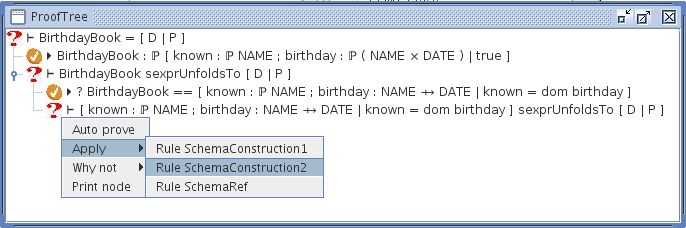
\includegraphics[width=\textwidth]{cztprover1}
  \caption{Screenshot of Interactive Prover}
  \label{fig:cztprover}
\end{figure}

The interactive prover shown in Figure~\ref{fig:cztprover} displays a
proof in tree form.  Each node is labelled with a subgoal.  If a rule
has been applied to a node, it can have children (instantiations of
the antecedents of the rule).  An icon indicates whether a node has
been proven (tick) or still needs to be proven (question mark).

The user can manipulate the proof tree by applying rules or oracles
and undoing rule and oracle applications.  Clicking on a node will pop
up a menu offering the choices available for that particular node.
For example, the menu for predicates to which no rule has been applied
offers the choice of ``Auto prove'' or to apply one of the matching
rules or oracles.  It also has a ``Why not'' submenu, which lists all
the rules and oracles that cannot be applied.  By selecting one of
those, the user gets detailed debugging information about why the
unification of the selected predicate and the conclusion of a
particular rule or oracle failed.

To provide the submenus ``Apply'' and ``Why not'', the prover goes
through all the known rules and oracles and tries to apply them to the
current predicate.  If this test application suceeds, the
corresponding rule or oracle name is added into the ``Apply''
submenu; if it fails, the name is added into the ``Why not''
submenu.  While this approach might be too inefficient and slow for
large rule sets, it has been very helpful for our purposes.

The ``Auto prove'' menu entry calls the automated prover described in
the next section.  If a proof is found, the resulting proof tree is
displayed as a subtree of the current node and the user can browse and
manipulate it.  Browsing a proof tree is eased by allowing subtrees to
be folded away by just clicking onto them.  If the mouse pointer is
above a particular node, the tooltip gives information about whether
and which rule or oracle has been applied.

This interactive prover is not intended to be a practical tool for
reasoning about Z specifications.  A much higher level of automation
would be needed for that.  But it has been found to be a very useful
tool in the development of rule sets for the other tools discussed
next.

\subsection{An Automated Depth-First Prover}

This tool is a Java class (called SimpleProver) that provides a
depth-first search method that can be used to find proofs
automatically.  Given a predicate, it tries to apply the rules and
oracles in the order they appear in the Z specification.  If a rule
application succeeds, a sequence of new subgoals is created and
attempted to be proven next (in the order provided by the rule).  If
proving the new subgoals fails, the next rule or oracle is tried
instead.  If an oracle application succeeds, the code for checking the
predicate is executed next.  If this succeeds, the predicate is
considered to be proven, otherwise the proof search is continued by
trying to apply the next rule or aracle.

Note that this simple prover uses a shallow backtracking algorithm and
therefore might fail to find a proof even when there exists one.  If a
proof for a subgoal is found, the prover sticks to it and no attempt
is made to find an alternative proof.  This might prevent another
subgoal from being proven.  Even though this approach is less general
than deep backtracking, this has not been a problem for the rules used
so far.  Furthermore, if a proof is found using shallow backtracking,
it is usually found more quickly than using deep backtracking.

\subsection{A Rewrite Engine} \label{sec:rewrite}

CZT also provides a Java class called Rewrite that can rewrite a given
Z term using a given set of rewrite rules.  A rewrite rule is a rule
whose conclusion is of the form $t1~r~t2$, where the left side $t1$
must match the term to be rewritten, the right side $t2$ represents
the result of the transformation, and $r$ is some equivalence relation
such as equality.  For example, the Rewrite engine will rewrite a Z
expression~$e1$ to the Z expression~$e2$ if it can prove $e1 = e2$
using repeated applications of rules from the given set of rewrite
rules.  Note that some rewrite rules may have antecedents, so applying
such rewrite rules can require proving any antecedent predicates --
the latter task is done using the SimpleProver tool mentioned earlier.

Usually, the task is to compute $e2$ for a given Z expression $e1$.
To do that, the rewrite engine asks the prover to prove $e1 = E$,
where $E$ is an expression joker.  The rewrite rules should be
designed so that, if a proof is found, the right-hand side of the
equation is ground, i.e.\ does not contain any unbound jokers.  Then
$e1$ is substituted by, or rewritten to, $e2$.

The rewrite engine is implemented by the Rewrite class, which provides
methods for rewriting expressions (using $e1 = e2$ rules) and
predicates (using $p1 \iff p2$ rules) once.  Another method combines
rewrites into sequences of rewrites and also considers subterms in a
top-down manner.  A given term is rewritten until it does not change
any more, and then its subterms are rewritten in the same way.

\section{Example Rules: Schema Unfolding and Normalisation} \label{sec:schemas}

\begin{zsection}
  \SECTION unfold \parents standard\_toolkit
\end{zsection}

This Z section contains rules for unfolding and normalising declarations
and schema expressions.  For example, given a schema expression such as $E
\land [x:\nat | p~x]$ where $E$ is the name of a schema, these rules define
an unfolding and normalisation process that will transform this schema
expression into an equivalent expression of the form $[D|P]$, where $D$ is
a list of variable declarations whose types are all carrier sets and $P$ is
a predicate that will contain constraints like $x \in \nat$ and $p~x$.

We start by declaring the jokers used in all the rules in this section.

\begin{zedjoker}{DeclList} D, D1, D2, D3, D4, D5, D6 \end{zedjoker}
\begin{zedjoker}{Pred} P, P1, P2, P3, P4, P5, P6 \end{zedjoker}
\begin{zedjoker}{Expr} T, E, E1, E2, E3, E4, E5, E6 \end{zedjoker}
\begin{zedjoker}{Name} v, v1, v2, v3, v4, v5, v6 \end{zedjoker}

Next we explain the oracles used.  We start with the type oracle that
can decide and compute the type of a given expression.  The syntax of
the oracle uses a relation defined as follows.

\begin{zed}
  \relation ( \_ \hasType \_ )
\end{zed}

\begin{gendef}[E1,E2]
  \_ \hasType \_ : E1 \rel E2
\end{gendef}

The type oracle gets an expression~$E$ and a carier set~$T$ (that is,
a Z expression that corresponds to a Z base type) and checks that $E$
is of type $T$.

\begin{zedproviso}{TypeOracle}
  E \hasType T
\end{zedproviso}

Note that $T$ is typically a joker, or contains jokers, in which case
the oracle calculates the type rather than just checking it.

The lookup oracle searches for a matching ConstDecl in the current Z
section and its ancestor sections.  It provides a way of looking up
definitions so that they can be used to unfold expressions.  The
left-hand side is usually a reference expression, which is a name plus
a list of expressions -- this allows generic definitions to be
instantiated and unfolded.  In the future we plan to expand this
lookup syntax, so that rules can query other kinds of Z paragraphs,
such as the declarations and predicates within axiomatic definitions.

\begin{zed}
  \relation (\_ \hasDefn \_)
\end{zed}

\begin{gendef}[E]
  \_ \hasDefn \_ : E \rel E
\end{gendef}

\begin{zedproviso}{LookupOracle}
  E1 \hasDefn E2
\end{zedproviso}

Calculate oracles use the relation $\is$ defined below.  They usually
calculate the left-hand side and then unify the result with the
left-hand expression.

\begin{zed}
  \relation (\_ \is \_)
\end{zed}

\begin{gendef}[E1,E2]
  \_ \is \_ : E1 \rel E2
\end{gendef}

An example is the schmema prime oracle that decorates a normalised
schema~$E$ and unifies the result of that computation with~$E2$.  Note
that this is less general than decorating an arbitrary schema
expression.

\begin{zedproviso}{SchemaPrimeOracle}
  E~' \is E2
\end{zedproviso}

Oracles for the other kinds of decorations can be given similarily.

The calculate theta oracle computes to a given theta expression like
$\theta~S$, where $S==[x,y:\nat]$, the binding expression $\lblot
x==x,y==y \rblot$.

\begin{zedproviso}{CalculateThetaOracle}
  \theta E \is E2
\end{zedproviso}

The $\schemaminus$ oracle subtracts one signature from another.  That
is, $D3$ will contain all the declarations that appear in $D1$ but do
not appear in $D2$.

\begin{zedproviso}{SchemaMinusOracle}
  [D1|true] \schemaminus [D2|true] \is [D3|true]
\end{zedproviso}

The $\unprefix$ oracle removes a word $v1$ from the front of the name
$v2$ and unifies the resulting name with $v3$.  It fails if $v2$ does
not start with $v1$.

\begin{zedproviso}{UnprefixOracle}
  v1 \unprefix v2 \is v3
\end{zedproviso}

\begin{zedproviso}{SortNamesOracle}
  (sort [D|true]) \is ([D1|true]? \land [D2|true]' \land
                       [D3|true]! \land [D4|true])
\end{zedproviso}


To clearly distinguish our rules for unfolding declaration lists and
schema expressions from other rules, we introduce two new infix
operators: $\sexprUnfoldsTo$ and $\declListUnfoldsTo$.  
We do not really need to define their semantics in order to use them within
rules, but to reassure readers, we define their semantics to be just
equality.  In fact, the intention is that the right-hand argument
will be the unfolded and normalized form of the left-hand argument.

\begin{verbatim}
%%Zinword \sexprUnfoldsTo sexprUnfoldsTo
%%Zinword \declListUnfoldsTo declListUnfoldsTo
\end{verbatim}
%
\begin{zed}
  \relation ( \_ \sexprUnfoldsTo \_ ) \\
  \relation ( \_ \declListUnfoldsTo \_ )
\end{zed}
%
% NOTE: we are using an old version of oz.sty that requires {T}, not [T]
\begin{gendef}{SCHEMA}
  \_ \sexprUnfoldsTo \_ : SCHEMA \rel SCHEMA \\
  \_ \declListUnfoldsTo \_ : SCHEMA \rel SCHEMA
\where
  \forall s1,s2:SCHEMA @ s1 \sexprUnfoldsTo s2 \iff s1=s2 \\
  \forall s1,s2:SCHEMA @ s1 \declListUnfoldsTo s2 \iff s1=s2 \\
\end{gendef}


\subsection{Unfolding Declaration Lists}

We use the $\declListUnfoldsTo$ operator for unfolding declaration
lists.  The left-hand side is always of the form $[DeclList|true]$ and
the right-hand side (which is usually a generated output) is of the
form $[D|P]$, where the declaration list $D$ contains variable
declarations only, has no duplicated names and all its expressions are
Z carrier sets, and the predicate $P$ contains any additional typing
constraints that were in DeclList.

The next few rules specify the $\declListUnfoldsTo$ operator.
The rules are intended to recurse through a declaration list from left
to right, with the base case of an empty declaration list being handled
by the EmptyDeclList rule.  Note that multiple declarations such as
$x,y,z:T$ are expanded out into separate declarations before rules
are applied, so the rules that follow cover all possible kinds
of declarations.

The VarDecl1 rule is a special case of VarDecl2.  It applies when $E$ is
already a carrier set.  Since VarDecl1 comes before VarDecl2 in this file,
the rewrite engine (see Section~\ref{sec:rewrite}) gives it higher
priority, and this avoids introducing redundant tautologies (such as $E \in
\arithmos$, which is guaranteed to be true by the type system) into the
predicate.  This is an example of how we can influence the behaviour of the
rewrite engine by placing more specific rules before more general ones.  Of
course, in the interactive prover, the user could choose to apply either
rule when $E$ is a carrier set.

\begin{zedrule}{VarDecl1}
   E \hasType \power E \\
   [D1 | true] \declListUnfoldsTo [D2 | P2]
\derives
   [v:E; D1 | true] \declListUnfoldsTo [v:E; D2 |  P2]
\end{zedrule}

\begin{zedrule}{VarDecl2}
   E \hasType \power E2 \\
   [D1 | true] \declListUnfoldsTo [D2 | P2]
\derives
   [v:E; D1 | true] \declListUnfoldsTo [v:E2; D2 |  v \in E \land P2]
\end{zedrule}

\begin{zedrule}{ConstDecl}
   E \hasType E2 \\
   [D1 | true] \declListUnfoldsTo [D2 | P2]
\derives
   [v==E; D1 | true] \declListUnfoldsTo [v:E2; D2 |  v = E \land P2]
\end{zedrule}

The IncludeDecl rule creates a subgoal $E \sexprUnfoldsTo \ldots$ that
will invoke the schema expression rules in the next section.  So the
two sets of $\declListUnfoldsTo$ and $\sexprUnfoldsTo$ rules are
mutually recursive.

\begin{zedrule}{IncludeDecl}
   E \sexprUnfoldsTo [D1 | P1] \\
   [D | true] \declListUnfoldsTo [D2 | P2] \\
   ([D1 | true] \land [D2 | true])\hasType \power [D3 | true] 
\derives
   [E; D | true] \declListUnfoldsTo [D3 |  P1 \land P2]
\end{zedrule}

\begin{zedrule}{EmptyDeclList}
   [~ | true] \declListUnfoldsTo [~ | true]
\end{zedrule}


\subsection{Unfolding Schema Expressions}

This section defines the unfolding of schema expressions,
using the $SE \sexprUnfoldsTo NORM$ operator, where $SE$
is a schema expression and $NORM$ is the resulting normalized
schema construction ($[Decls|Preds]$, where the types in $Decls$
are only carrier sets).

The TopLevel rule is an equality rewrite rule for expressions.  The
type oracle ensures that it is applicable only when $E$ is a schema
expression.  The last antecedent uses the $\sexprUnfoldsTo$ rules in
this section to rewrite $E$ to $[D | P]$.

\begin{zedrule}{TopLevel}
  E \hasType \power [D2 | true] \\
  E  \sexprUnfoldsTo [D | P]
\derives
  E = [D | P]
\end{zedrule}

The Theta rule rewrites expressions into a binding.  The type
oracle is used to calculate the signature of $E$, then the theta
oracle generates the appropriate binding expression from that
signature.
\begin{zedrule}{Theta}
  E \hasType \power [D | true] \\
  \theta [D | true] \is E2
\derives
  \theta E = E2
\end{zedrule}


The next rule handles decorated $\theta$ expressions.  However, this
version handles only a single prime decoration.  We need thirteen
versions of this next rule -- one for 
each possible decoration.   In the future we will extend the ZedRules
notation to support Stroke-List jokers, so that all decoration lists can
be handled by a single rule.

\begin{zedrule}{ThetaPrime}
  E \hasType \power [D | true] \\
  \theta [D | true] ' \is E2
\derives
  \theta E~' = E2
\end{zedrule}

Like VarDecl1 and VarDecl2, the SchemaConstruction1 rule is a special
case of SchemaConstruction2.  It applies to schemas that are already
normalised and avoids adding lots of redundant typing conditions into
the predicate part.
\begin{zedrule}{SchemaConstruction1}
  [D1 | true] \declListUnfoldsTo [D2 | true]
\derives
  [D1 | P] \sexprUnfoldsTo [D2 | P]
\end{zedrule}

\begin{zedrule}{SchemaConstruction2}
  [D1 | true] \declListUnfoldsTo [D2 | P2]
\derives
  [D1 | P] \sexprUnfoldsTo [D2 | P2 \land P]
\end{zedrule}

The SchemaRef rule uses the lookup oracle to unfold schema names
($E$ may specify an instantiation of a generic schema).  
The result of the lookup
is then normalised to obtain the overall result.
\begin{zedrule}{SchemaRef}
  E \hasDefn E2 \\
  E2 \sexprUnfoldsTo [D2 | P2]
\derives
  E \sexprUnfoldsTo [D2 | P2]
\end{zedrule}

This rule unfolds any remaining $\Delta$ schemas.  If the
specification explicitly defined the $\Delta$ schema, then the above
SchemaRef rule would have unfolded it.  There is a similar rule for
$\Xi$ schema names.

\begin{zedrule}{DeltaRef}
  \Delta \unprefix v \is v2 \\
  [v2; v2~'] \sexprUnfoldsTo [D1|P1]
\derives
  v \sexprUnfoldsTo [D1|P1]
\end{zedrule}


The SchemaPrime rule uses the schema prime oracle to decorate a
normalised schema.  Note that we also currently need thirteen versions
of this next rule -- one for each possible decoration.

\begin{zedrule}{SchemaPrime}
   E \sexprUnfoldsTo [D1 | P1] \\
   [D1|P1]~' \is [D2|P2] \\
\derives
   E~' \sexprUnfoldsTo [D2 | P2]
\end{zedrule}

The type oracle in the ExistsSchema rule checks that $D1$ and $D2$ are
type compatible.  The $\schemaminus$ oracle subtracts $D1$ from~$D2$.
The rule for schema $\forall$ is similar.

\begin{zedrule}{ExistsSchema}
   [D|P] \sexprUnfoldsTo [D1 | P1] \\
   E2 \sexprUnfoldsTo [D2 | P2] \\
   ([D1 | true] \land [D2 | true]) \hasType \power [D3 | true] \\
   ([D2|true] \schemaminus [D1|true]) \is [D4|true]
\derives
   (\exists D | P @ E2) \sexprUnfoldsTo [D4 | (\exists D1 @ P1 \land P2)]
\end{zedrule}

The semantics of schema negation requires schemas to be
normalised before their predicate is negated.

\begin{zedrule}{SchemaNegation}
  E \sexprUnfoldsTo [D | P]
\derives
  (\lnot E) \sexprUnfoldsTo [D | \lnot P]
\end{zedrule}

The SchemaConjunction rule is straightforward -- it uses a type
oracle to check that the signatures of the two schemas are compatible.
The schema disjunction, implication and equivalence rules are similar.

\begin{zedrule}{SchemaConjunction}
  E1 \sexprUnfoldsTo [D1 | P1] \\
  E2 \sexprUnfoldsTo [D2 | P2] \\
  ([D1 | true] \land [D2 | true]) \hasType \power [D3 | true]
\derives
  (E1 \land E2) \sexprUnfoldsTo [D3 | P1 \land P2]
\end{zedrule}

Schema projection, $E1 \project E2$, is also similar to schema conjunction,
but the resulting schema has only the names that are declared in $E2$.
Any other names that are declared in $E1$ are hidden existentially.

\begin{zedrule}{SchemaProjection}
  E1 \sexprUnfoldsTo [D1 | P1] \\
  E2 \sexprUnfoldsTo [D2 | P2] \\
  ([D1 | true] \land [D2 | true]) \hasType \power [D3 | true] \\
  ([D3 | true] \schemaminus [D2 | true]) \is [D4 | true]
\derives
  E1 \project E2 \sexprUnfoldsTo [D2 | (\exists D4 @ P1 \land P2)]
\end{zedrule}

To calculate the precondition of a schema, we must existentially
hide all the output names, such as $x!$ or $x'$.  The $postnames$ 
operator in the following rule takes a normalised schema as input and
returns (in $D2$) just the declarations whose names have a final decoration 
of $!$ or $'$.  These names are removed from $D4$, so that $D3$ contains 
only the declarations of names that should appear in the precondition, 
such as $x$, $x?$ and $x_2$.

\begin{zedrule}{SchemaPrecondition}
  E \sexprUnfoldsTo [D4 | P2] \\
  (sort [D4|true]) \is ([D6|true]? \land [D7|true]' \land
                        [D8|true]! \land [D9|true]) \\
  ([D6|true]? \land [D9|true]) \hasType \power [D1|true]
\derives
  \pre E \sexprUnfoldsTo [ D1 | (\exists ([D7|true]' \land [D8|true]!) @ P2)]
\end{zedrule}

Schema composition is one of the most complex schema operators.
Note that $\bowtie$ is a special decoration that cannot be entered by
users.

\begin{zedrule}{SchemaComposition}
  E1 \hasType \power [D1 | true] \\
  E2 \hasType \power [D2 | true] \\
  (sort [D1|true]) \is ([D6|true]? \land [D4|true]' \land
                        [D8|true]! \land [D9|true]) \\
  ([D4 | true] \schemaminus [D2 | true]) \is E5\\
  ([D4 | true] \schemaminus E5) \is E6 % matching names
\derives
  E1 \semi E2 =
  (\exists E6~\bowtie @ (\exists E6~' @ [E1 | \theta E6~' = \theta E6~\bowtie])
                   \land
                   (\exists E6   @ [E2 | \theta E6   = \theta E6~\bowtie]))
\end{zedrule}

%TODO: schema hiding, schema piping, schema exists unique.


%\subsection{Rules for Unfolding Quantified Declarations}
%
%When rewriting terms involving quantifiers, we want to
%rewrite and expand the schema text $E$ within quantifiers
%such as $\exists E @ P$ or $(\lambda E@E2)$, as well as rewriting
%the predicates and expressions within the body of the quantifiers.
%The rewrite tactics try to transform such schema text using the 
%$\schemaEquals$ relation.  So the following rule applies the above 
%schema unfolding rules to unfolding any schema text that appears within 
%the bound variable part of quantifiers.
%\begin{zedrule}{Quantifiers}
%   [D|P] \sexprUnfoldsTo [D1|P1]
%\derives
%   [D|P] \schemaEquals [D1|P1]
%\end{zedrule}


\subsection{Rules for Unfolding Schemas as Predicates}

If a schema expression $E$ is used as a predicate, it is equivalent to
checking that $\theta E$ (a binding constructed from names that are
currently in scope) satisfies the predicate part of $E$ 
(including any subtypes in the declarations).  So this rule
transforms any expression that is used as predicate into $\theta E \in E$.
\begin{zedrule}{SchemaPred}
  E \iff \theta E \in E
\end{zedrule}


\section{Example Rules: ZLive Preprocessor} \label{sec:zlive}

In this section we show just a few of the rules that the ZLive
animator uses to unfold and simplify Z expressions before starting
animation.  When an expression is given to ZLive to animate, the first
phase of animation (after parsing and typechecking) is to use the CZT
Rewrite Engine (see Section~\ref{sec:rewrite}) to apply the following
set of rules to the expression.

\begin{zsection}
  \SECTION ZLivePreprocess \parents unfold
\end{zsection}

Note that this $ZLivePreprocess$ section has the $unfold$ section (see
Section~\ref{sec:schemas}) as a parent, so the schema unfolding rules
from the $unfold$ section are effectively the first rules in the
$ZLivePreprocess$ section.  If we wanted to reuse multiple rule sets,
we could simply list multiple parents, in the desired order.

The SchemaToSet rule unfolds schemas that are used as expressions into
set comprehensions.  Since this rule appears \emph{after} the schema
rule from the $unfold$ section, schema expressions will be unfolded
and normalised before this rule is applied. 
\begin{zedrule}{SchemaToSet}
[D | P] = \{ D | P @ \theta [D | true] \}
\end{zedrule}

The next two rules are adapted from the sets toolkit and the
relations toolkit of the Z standard.  They illustrate how rewrite rules
can be used to unfold one operator and express it in terms of other
simpler operators.  ZLive needs no builtin knowledge of intersection
or $\dom$ -- these two rules are all that is needed.  Around 40 of the
standard toolkit operators are unfolded by rules in this way.

\begin{zedrule}{intersection}
   E1 \cap E2 = \{x:E1 | x \in E2\}
\end{zedrule}
\begin{zedrule}{domain}
   \dom E = \{x:E @ x.1\}
\end{zedrule}

We finish this section with a rather bizarre use of rules.  ZLive uses
an internal data structure, RelSet, to represent function and relation
spaces, such as $\nat \fun \{0,1\}$.  This data structure records the
domain and range set, plus various flags according to the properties
of the function space (total, onto, functional, injective).  This
gives a compact representation of the function space and makes it easy
to efficiently check if a given set of pairs is a member of the
function space or not.  The following two rules illustrate how the the
Z function space operators are rewritten into strange $\LET$ terms,
which ZLive recognises and converts into a RelSet object.  These rules
are not true equalities, but are used to rewrite a term like $\nat
\fun \{0,1\}$ into the temporary $\LET$ form, which is then translated
into a RelSet object that is equivalent to $\nat \fun \{0,1\}$.

\begin{zedrule}{fun}
   E1 \fun E2 = (\LET isFun==1;isTotal==1 @ \power (E1 \cross E2))
\end{zedrule}
\begin{zedrule}{bij}
   E1 \bij E2 = (\LET isFun==1;isTotal==1;isOnto==1;isInj==1 \\
   \t3               @ \power (E1 \cross E2))
\end{zedrule}

Using rules to preprocess expressions and unfold schemas has made it
far faster to develop ZLive and makes it easier to experiment with
alternative translations of an operator.


\section{Conclusions} \label{sec:concl}

We have described the ZedRules notation and illustrated its utility
for schema normalisation and general rewriting.  The main advantage
of the notation is that it is a superset of standard Z and it makes it
much easier and clearer to develop Z tools that perform non-trivial
transformations.


In the future, we would like to be able to extend the ZedRules
notation to fully support a variety of Z logics, such as
$\Zc$~\cite{henson:revising-z-1-99,henson:revising-z-2-99},
$\V$~\cite{brien:calculus-schemas-z00} (a successor of the
$\mathcal{W}$ logic that appeared in early drafts of the Z standard).
It is desirable to support both $\Zc$ and $\V$ (and any future
proposals for Z logics), since they are rather different and it would
be interesting to compare them in a common framework.  For example,
substitution is a meta-level operation in $\Zc$ but is defined within
the object logic of $\V$.  To support richer logics such as these, it
would be necessary to generalise antecedents into sequents that can
specify a different context to that of the conclusion.  For example,
an antecedent such as $x:T \vdash P$ would allow the proof of $P$ to
proceed in an extended context where the new variable $x$ is declared
and has type $T$.  This is similar to the common sequent calculus
style of proof~\cite{girard:proofs-types90}.

The current CZT reasoning tools construct an explicit proof tree that
allows proofs to be recorded, replayed, displayed, checked by independent
tools etc.
It would be interesting to build a tactic layer on top of this proof
tree, using a tactic language such as ANGEL~\cite{martin:tactics}, which
has been used as the basis of several other Z provers
(CADiZ~\cite{Toyn98a}, Jigsaw1, Jigsaw2,
Ergo~\cite{martin:tac-lang-for-ergo}).
This would make it easier to program combinations of rules 
in flexible ways, whereas currently such tactics must be written as
Java methods.
If ZedRules was extended to support richer logics and the CZT tools were 
extended to support tactics, they could be used as practical Z theorem
provers (after a large amount of theory development).

In the future, we would also like to be able to translate rules
into a form that existing Z theorem provers can accept, so that we can prove
rules correct and prove that a given set of rules preserves the Z
semantics.  A simple declarative semantics for rules makes this
easier to achieve.

\bibliographystyle{entcs}
\bibliography{spec,logic,thmprove,misc,proceedings}
\end{document}
